\documentclass[twocolumn]{article}
\usepackage[toc,page]{appendix}
\usepackage{amsmath}
\usepackage{graphicx}
\usepackage{subfloat}

\graphicspath{{./figures}}

\title{Thermoshit of Rocket Fuckups during disasterous flight}
\author{Eric Souder}
\date{July 2022}
\twocolumn

\begin{document}
    \maketitle
    \begin{abstract}
    \end{abstract}
    \section{Introduction}
        During the launch of a sounding rocket, the exterior of the vehicle experiences
        heat loading, etc etc idk

    \section{Modeling Nosecone Skin Heating}
        Objects traveling at high speeds are subject to heating and cooling as 
        they travel through the atmosphere. As a rocket vechile travels at 
        supersonic velocities, there are two signigigant contributions to 
        the temperature change of the nosecone - the aerodyanmic heating from 
        the compression of air as the nosecone pushes through it, and the heat
        lost to the atmosphere through radiation. For the purposes of this 
        analysis, these will be the only sources of thermal energy change
        considered.
        \subsection{Nosecone Aerodynamic Heating}
            As the nosecone travels at suspersonic speeds, it forms a shock wave
            as it moves faster than the air can escape. This can also be
            considered as air being blown towards a stationary nosecone, at the
            speed the rocket would be travling. At the very tip of
            the nosecone, the air has zero relative velocity to the vehicle. 
            This is the stagnation point [REF!].

            At the stagnation point, all of the kinetic energy of the air is 
            converted into thermal energy. Becuase this process happens so
            quickly, it can be modeled as an adiabatic compression of gas.

            \[PV^\gamma = \textrm{constant}\]

            The ideal gas approximation ($V\propto TP^{-1}$) can be applied, so 

            \[P^{1-\gamma}T^\gamma=\textrm{constant}\]

            In our compression, this means 

            \[\frac{T_s}{T_0}=\left(\frac{P_s}{P_0}\right)^\frac{\gamma-1}{\gamma}\]

            With $T_s, P_s$ as the stagnation temperature and pressure and 
            $T_0, P_0$ as the static temperature and pressure. The relation 
            between the static and stagnation pressure of a gas is sourced from 
            a National Adivosry Committee for Aeronautics report on compressable 
            flow:
            %https://www.grc.nasa.gov/WWW/BGH/Images/naca1135.pdf, eqn 44%

            \[\frac{P_s}{P_0} =\left(1+\frac{\gamma-1}{2}M^2\right)^{\frac{\gamma}{\gamma-1}}\]

            Where $M$ is the mach number. This provides an equation for
            stagnation temperature as a function of speed:

            \[\frac{T_s}{T_0}=1+\frac{\gamma-1}{2}M^2\]

            Of course, the entire nose cone will not encounter air at the
            stagnation temperature. Most air will be slowed, but stopped by skin 
            friction with the vehicle. Toft [citatation!]
            %http://dark.dk/documents/technical_notes/simplified%20aerodynamic%20heating%20of%20rockets.pdf%
            %might be more accurate to use NACA or something citation here, see toft's citation%
            models the temperature of the boundary layer air ($T_B$) based on
            $K$, a temperature recovery factor:

            \[K=\frac{T_B-T_0}{T_s-T_0}\]

            Eber [citation] provides a value of $K=0.89$ for cones with vertex
            angles between 20 and 50 degrees.

            We then have an equation for the temperature of the boundary layer:

            \[T_B=KT_s+T_0\left(1-K\right)\]

            Eber also provides an experimentally modeled value for $h$, the heat
            transfer function:
            
            \[h=\left(0.0071+0.0154 \sqrt[2]{\beta}\right)\frac{k}{\mu^{0.8}l^{0.2}}\left(\rho_0 u\right)\]

            based on $k$, the thermal conductivity of air; $\beta$, the vertex 
            angle of the cone; $\rho$, the density of the air; $\mu$, the dynamic
            viscosity of air; $u$ the velocity of the rocket; and $l$, the 
            length of the cone measured along the surface. 

            With all this, we can determine the heat flux into the nosecone skin
            from aerodynamic effects:

            \begin{equation}
                \dot{Q}_{aero}= h(T_B-T_N)
            \end{equation}

            Where $T_N$ is the actual temperaure of the nosecone skin.

        \subsection{Radiative Effects}
            Some amount of heat flux leaves the nosecone as blackbody radiation,
            with heat flux $\dot{Q}_rad=\epsilon\sigma(T_0^4-T_N^4)$, where
            $\epsilon$ is the emmisivity of stainless steel nosecone and 
            $\sigma$ is the Stefan-Boltzman constant.

            %talk about absorption of solar radiation?%

        \subsection{Flight Profile}
            In order to model the thermal behavior of the nosecone, we must
            provide a number of inputs to our aerodynamic heating simulation 
            functions based on altitude and velocity. These inputs are provided 
            by UBC Rocket's proprietary Feynman vehicle design program.
            
            Although Feynman was originally intended for optimizing the design
            of rocket vechicle components, such as fins, engines, or nosecones 
            for maximum altitude without regard for thermal effects, its outputs
            are helpful in the analysis of the nosecones thermal properties. 

            Feymnman provides data for Mach number and altitude at 10
            millisecond intervals for the first approximately 160 seconds of
            flight, corresponding to a peak altitude of almost 100 kilometers. 
            For this reason, we can use the output data of the Feynman
            simulaiton as a reasonable input flight profile for our thermal
            analysis.

            \begin{subfigures}
                \begin{figure}[h]
                    \label{fig:alt}
                    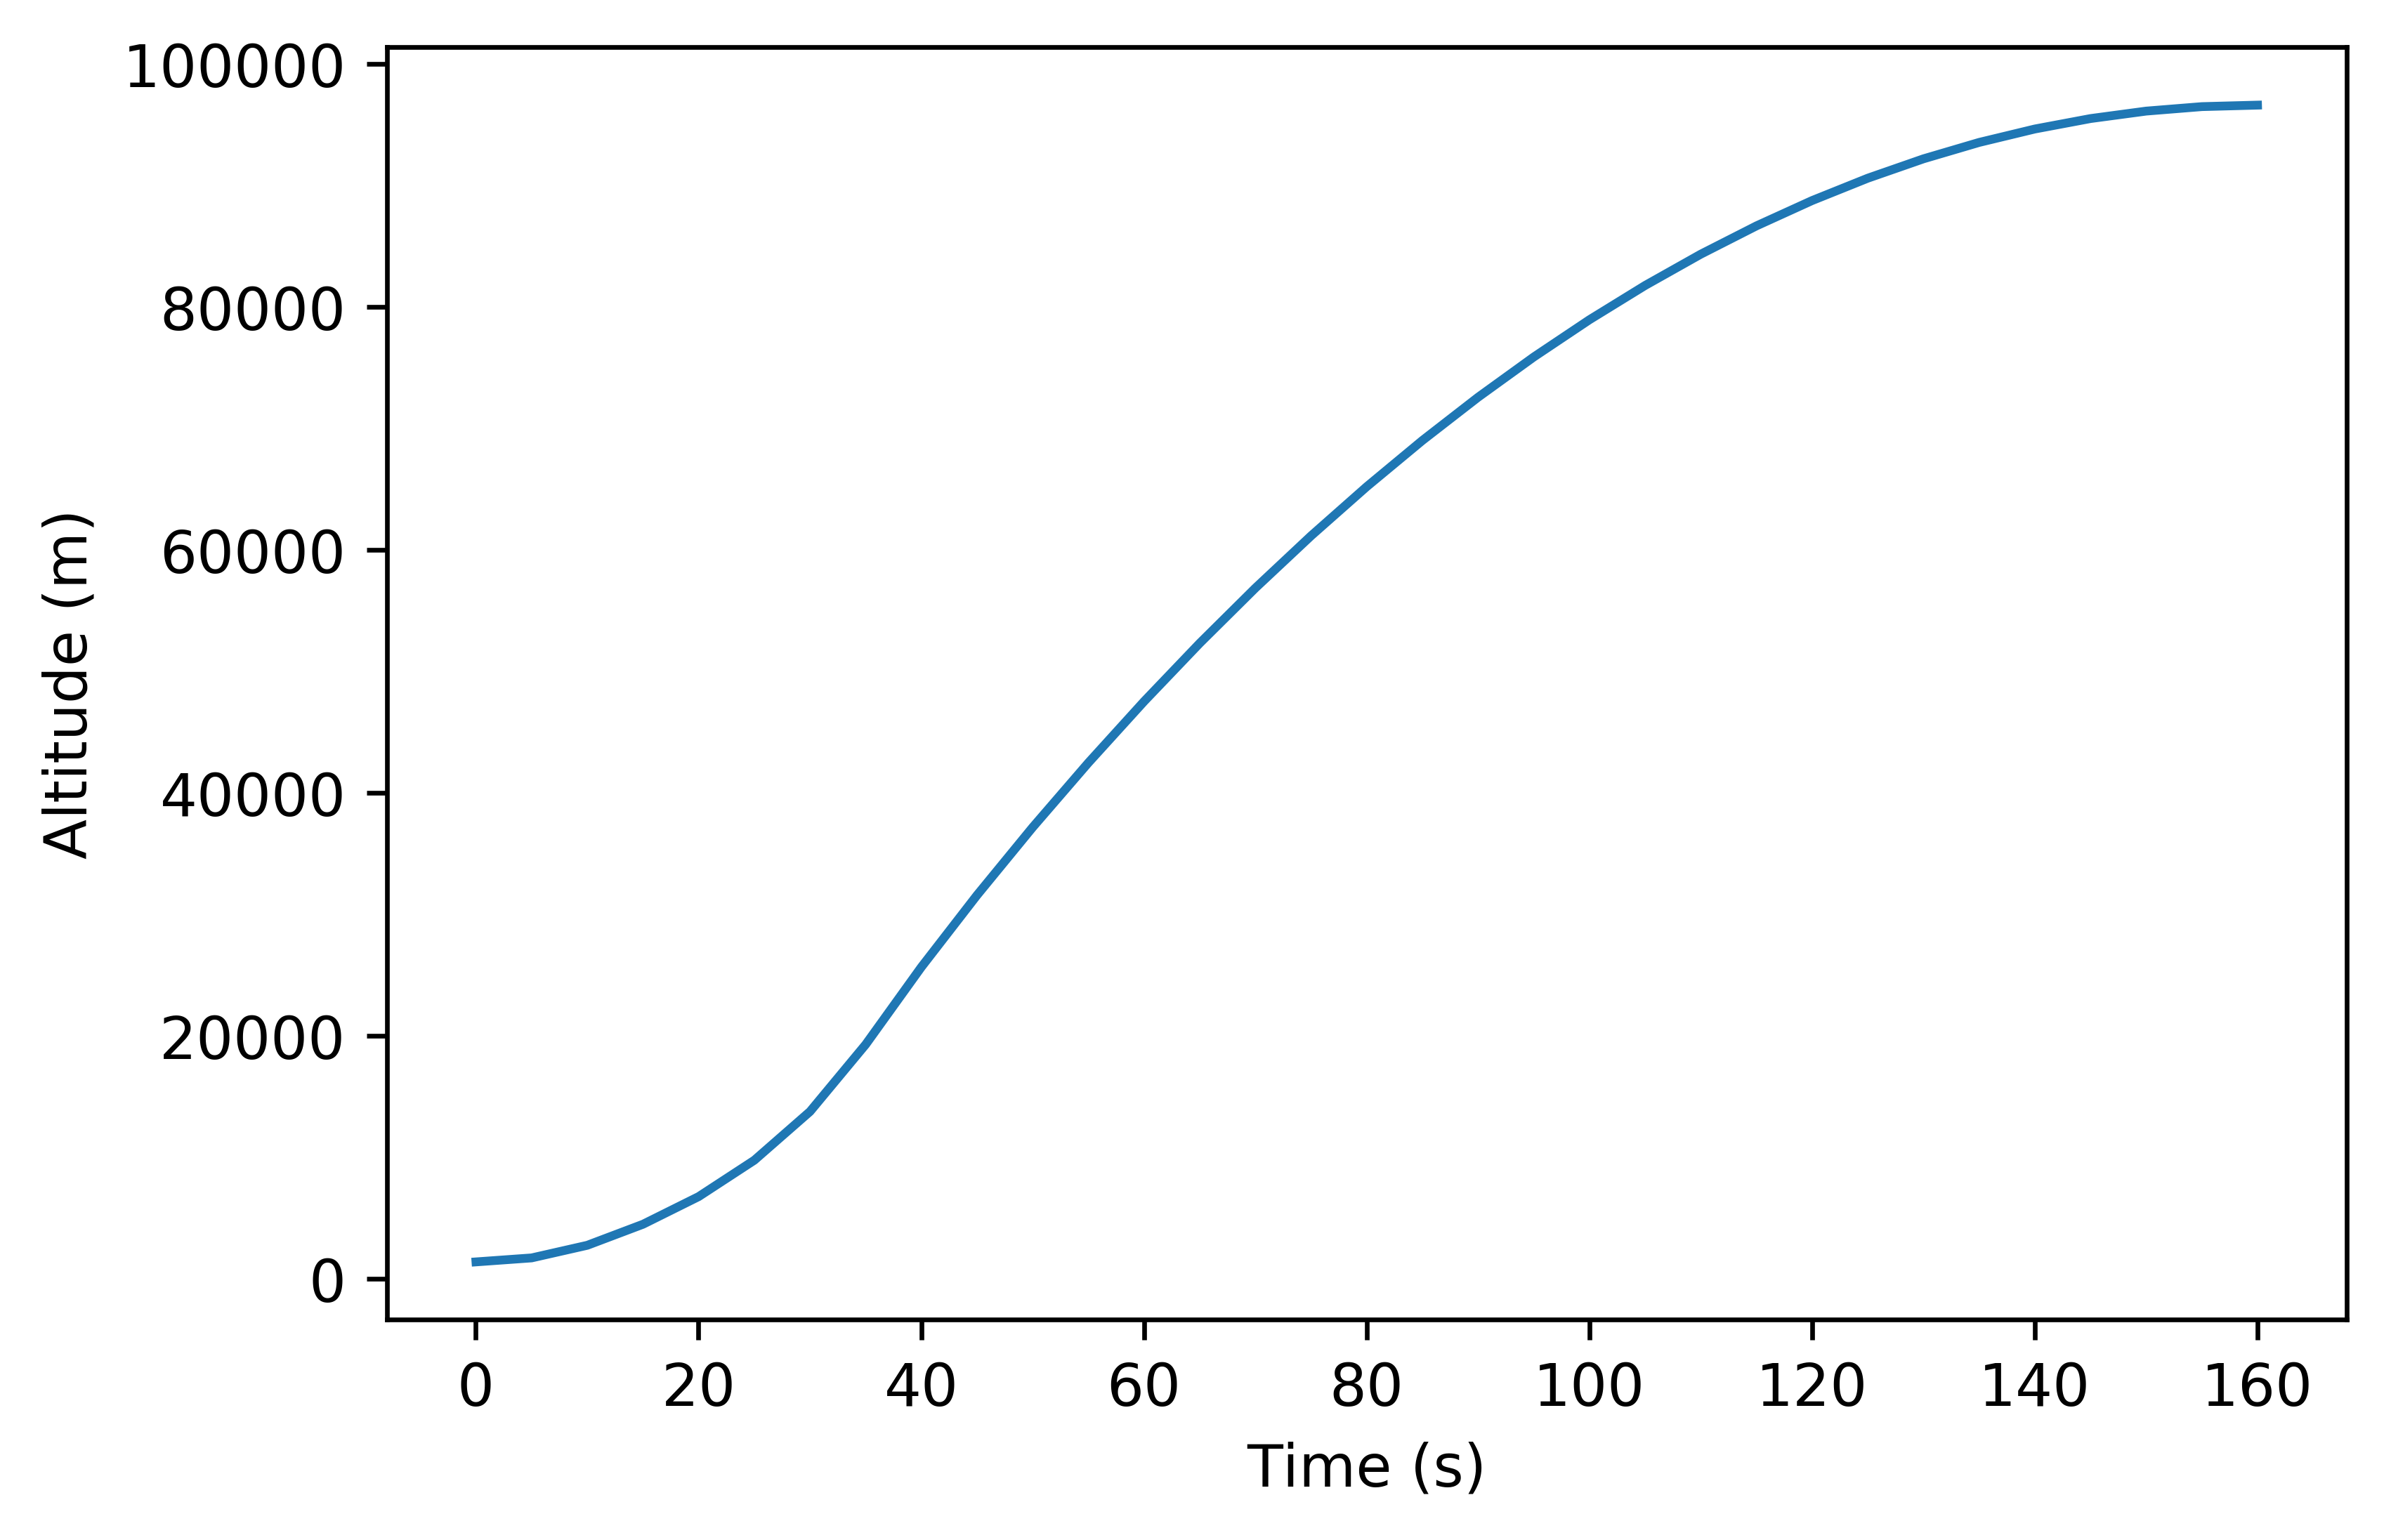
\includegraphics[width=\linewidth]{altitude.png}
                    \caption{Altitude vs Time of simulated vehicle trajectory}
                \end{figure}
                \begin{figure}[h]
                    \label{fig:mach}
                    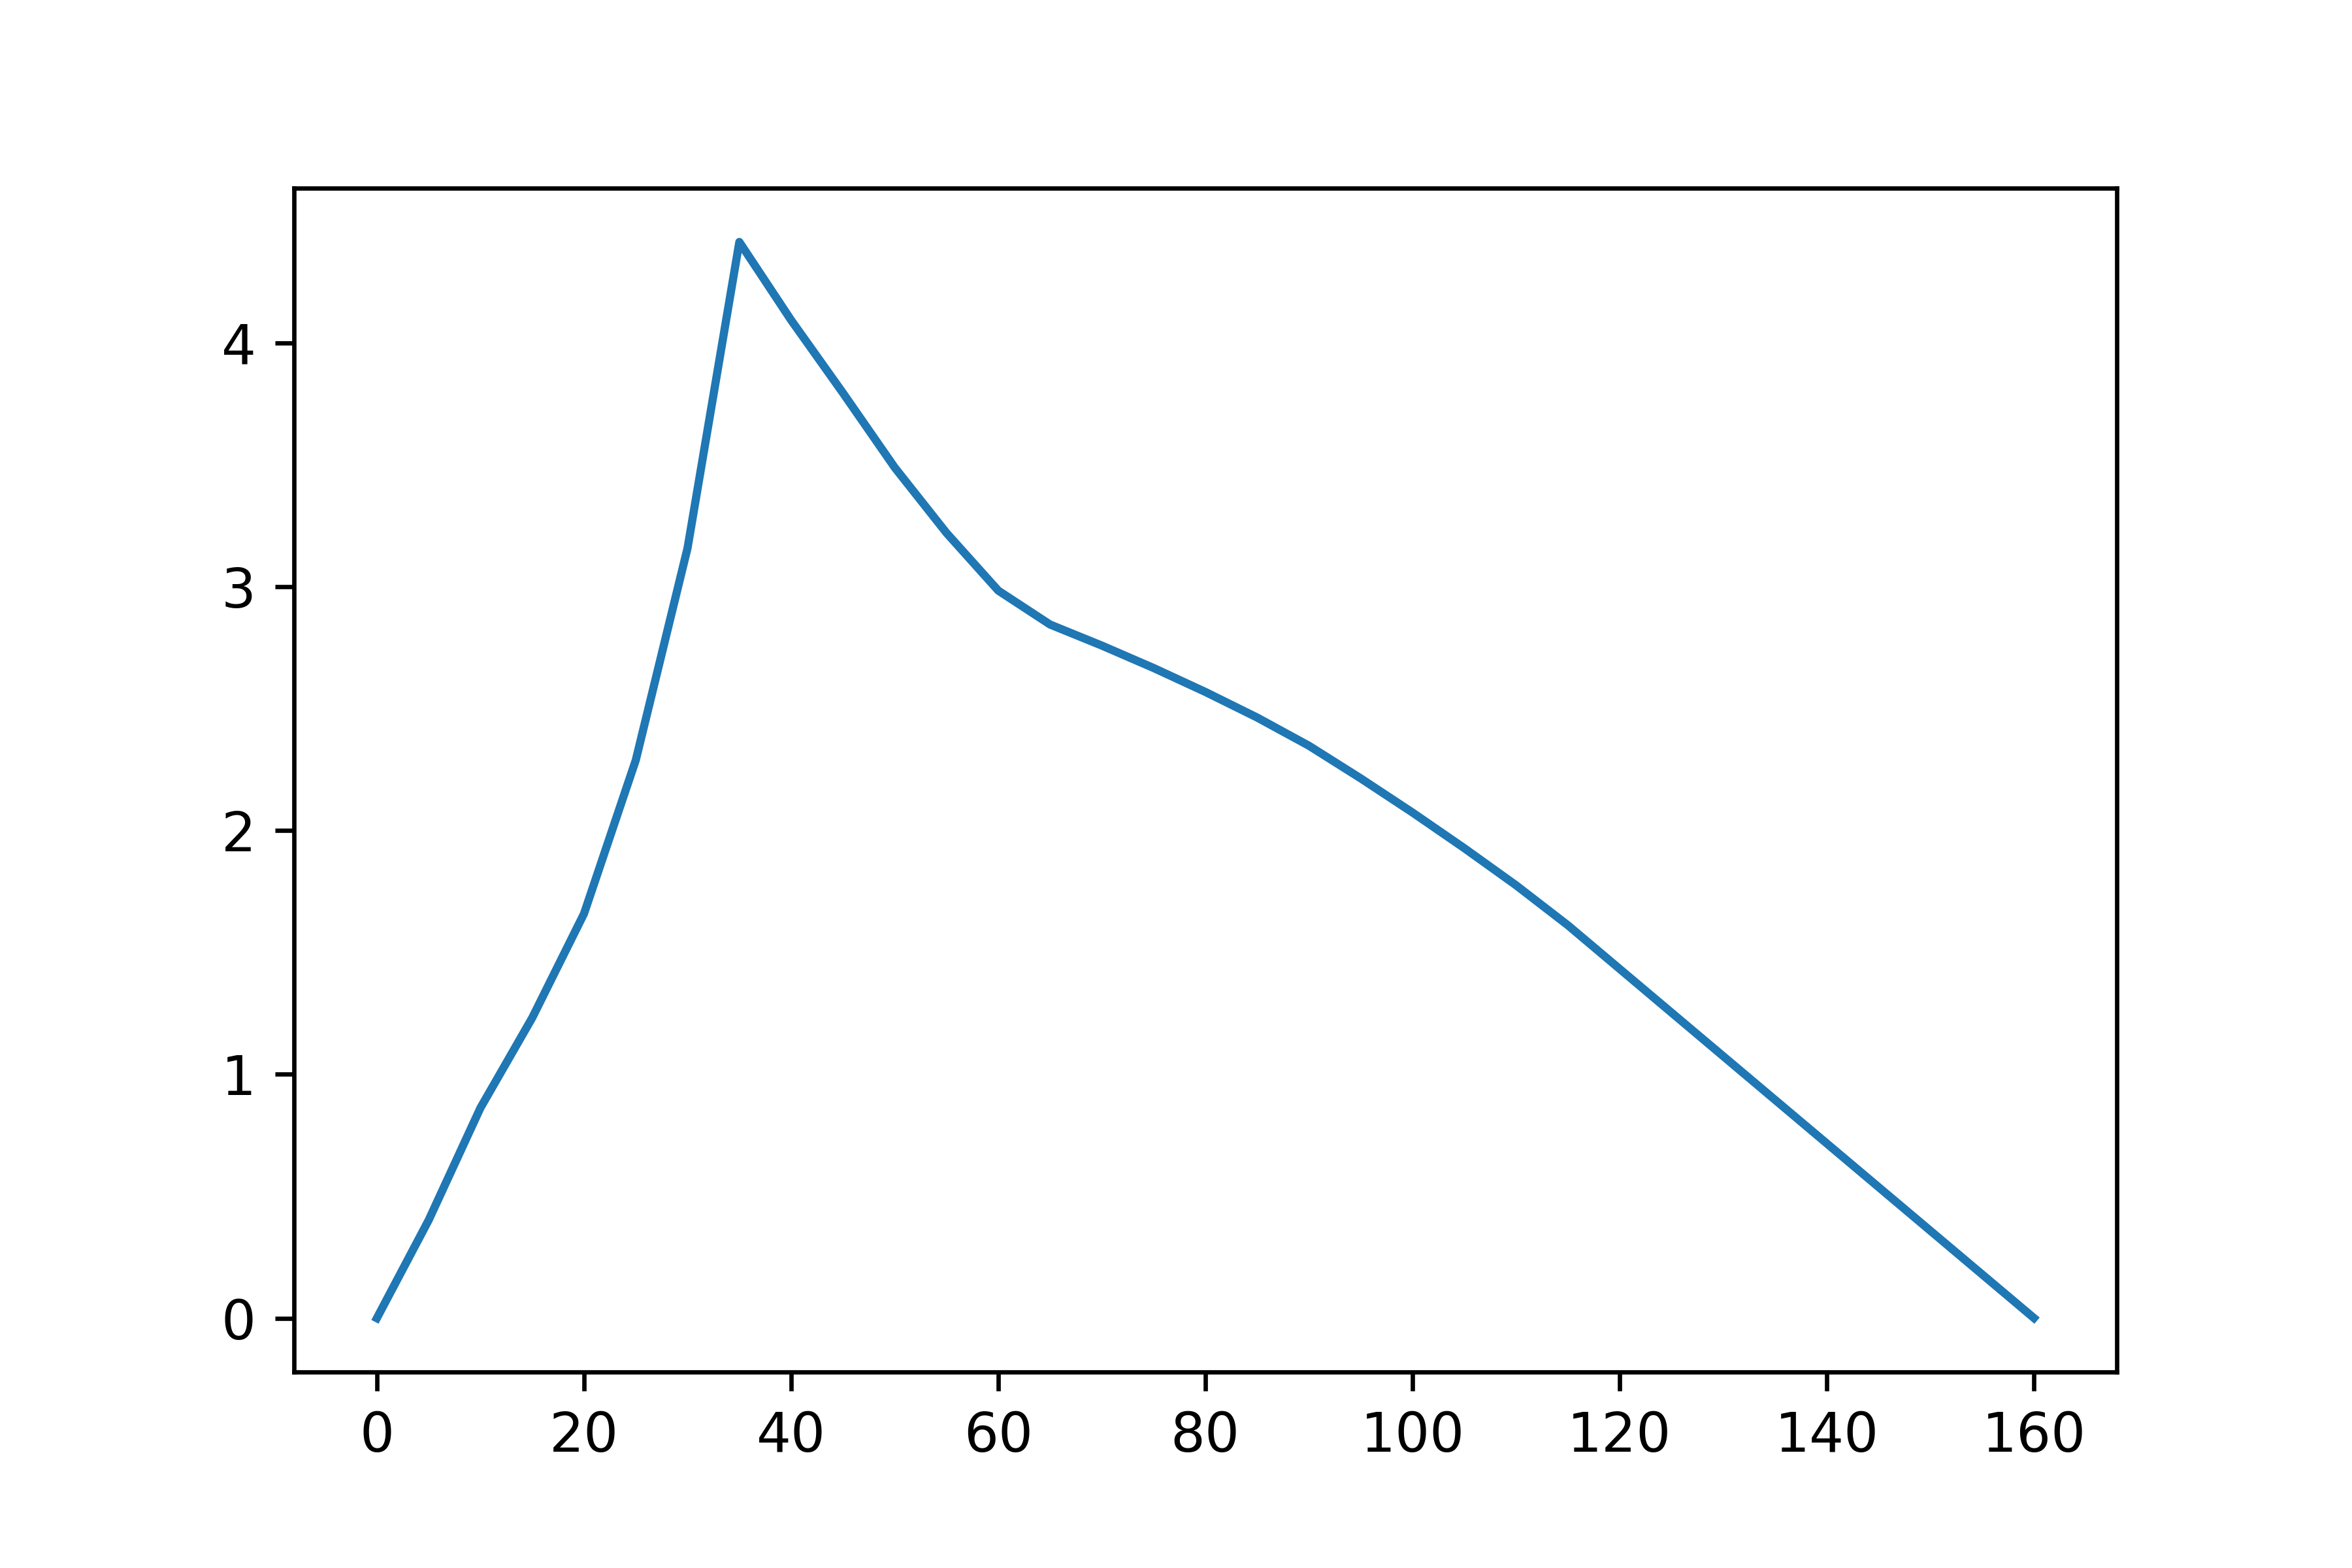
\includegraphics[width=\linewidth]{machs.png}
                    \caption{Mach number vs time of simulated vechicle trajectory}
                \end{figure}
            \end{subfigures}

            Additionally, emperically-derived curves\footnote{
                Unfortunately, some of this data was emperically-derived in Nazi 
                Germany by scientests working on the V-2 missile.}
            for $\rho_0$ and  $T_0$ in 
            terms of altitude and of $\mu$ and $k$ in terms of $T_0$ are 
            provided in appendix \ref{appendix:a}. These provide a full picture
            of the conditions around the nosecone over all stages of the flight.
        \subsection{Heat Flux Balance}
            The nosecone situation through flight can be modeled by an energy 
            balance:

            \[\textrm{Heat Flux In} = \textrm{Heat Flux out}\]

            This can be modeled by the heat equation:

            \[G dT_N = dt(\dot{Q}_{aero}-\dot{Q}_{rad})\]

            or 

            \begin{equation}
                \label{dTN}
                dT_N = \frac{dt(\dot{Q}_{aero}-\dot{Q}_{rad})}{G}
            \end{equation}

            With a factor $G$, the 'skin heating capacity' [cite] % note cite toft's [1] source or toft%
            determined by the specific heat of the nosecone skin $c$, it's 
            thickness $\tau$, and it's density $\rho$.

            \[G=c\tau\rho\]

        \subsection{Simulation Method}

            Considering a small but finite change in time $\Delta t$ (in our 
            simulation case, $10ms$, from Feynman as above), we can
            numerically solve for the change $\Delta T_N$ in the nosecone
            temperature based on equation \ref{dTN} above. 

            This solution is determined by means of a python simulation which
            iterates over each timestep and calcuates the change in $T_N$
            for that time. Using the atmospheric models from appendix 
            \ref{appendix:a} and the constant values from appendix 
            \ref{appendix:b}, a represntative model of the at-rest (i.e. far
            away from the vehicle's path of flight) is created. Then, using the 
            Feynman-derived data for Mach number and altitude, and the derived
            equations from the above sections, values are determined for $u,
            \mu, k, h, T_s, T_B, \dot{Q}_{aero}$ and $\dot{Q}_{rad}$, which are
            then used to solve for $\Delta T_N$ for the timestep, which then
            modifies $T_N$ for use in the simulation of the next timestep.

        \section{Discussion of Results}

            \begin{figure}[h]
                \label{fig:temptime}
                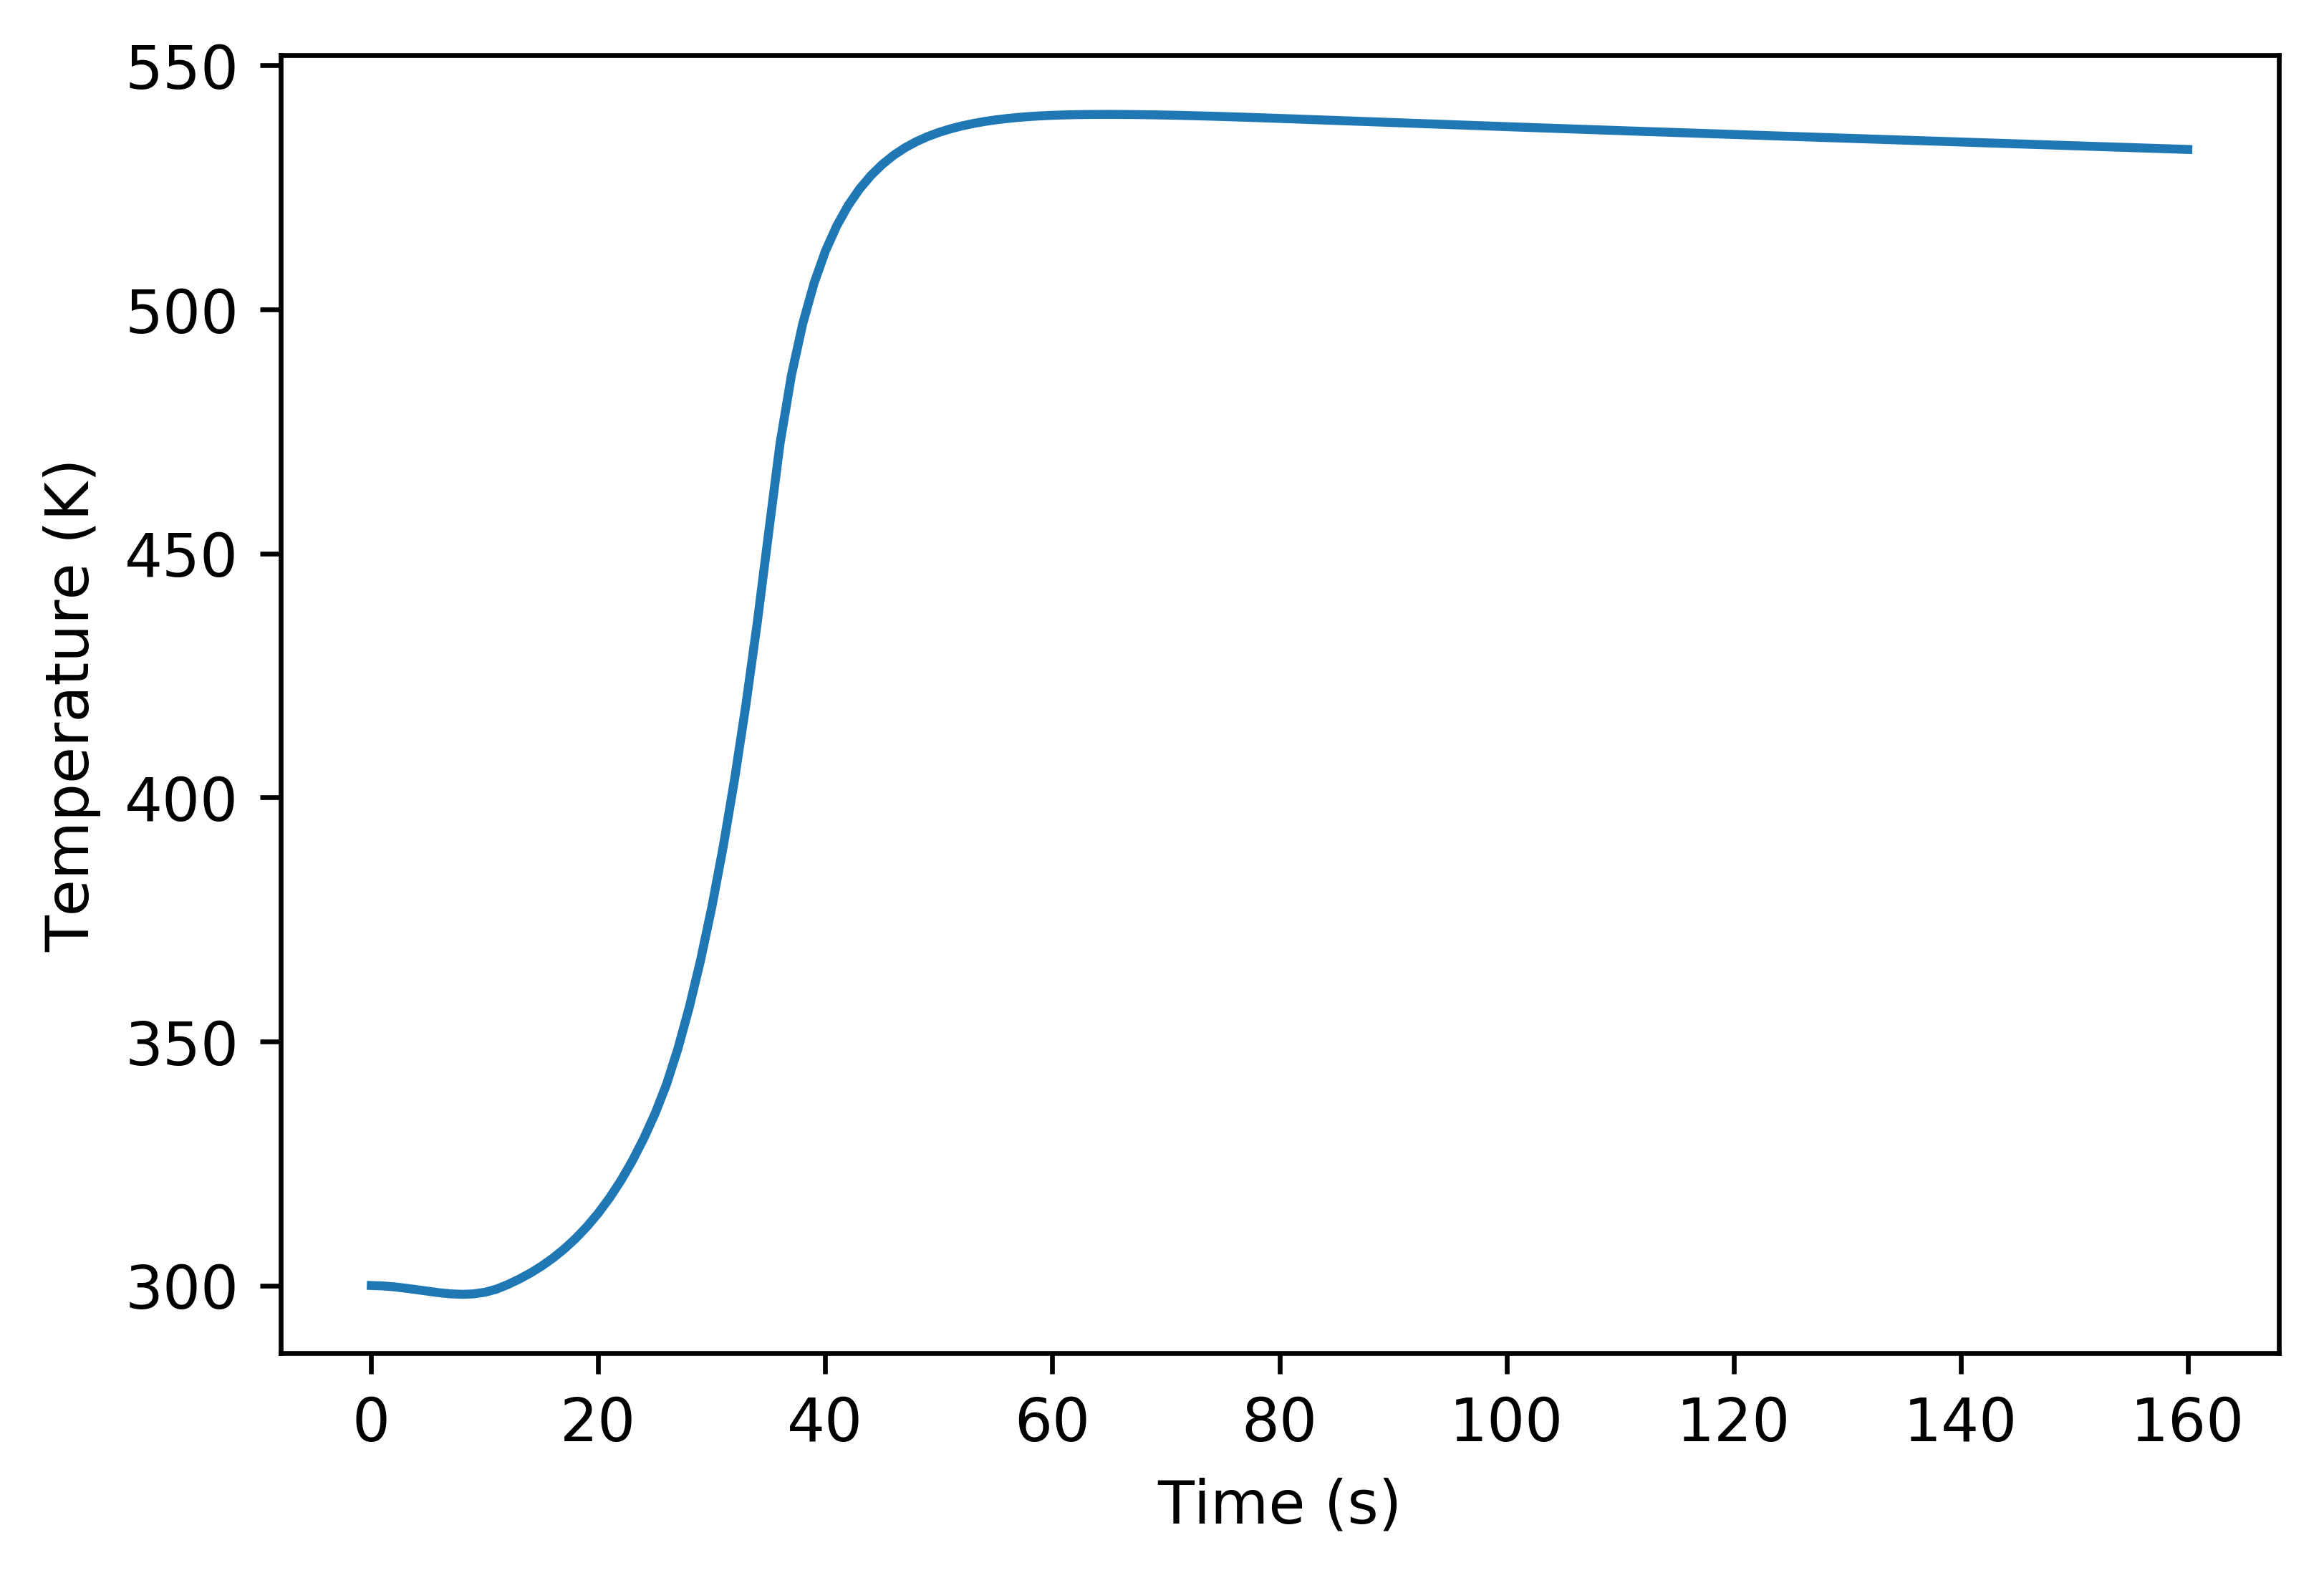
\includegraphics[width=\linewidth]{tempprofile.png}
                \caption{Temperature of nosecone skin vs time}
            \end{figure}

            Based on the above simulation, the temperature of the nosecone can
            be determined as a function of time as seen in figure 
            \ref{fig:temptime} above. The peak temeperature of 348 K occurs
            about 65 seconds into the flight. It is interesting to note that 
            after the rapid rise in temperature, the decline after the peak is 
            signifigantly shallower. 
                         

            \begin{figure}[h]
                \label{fig:flux}
                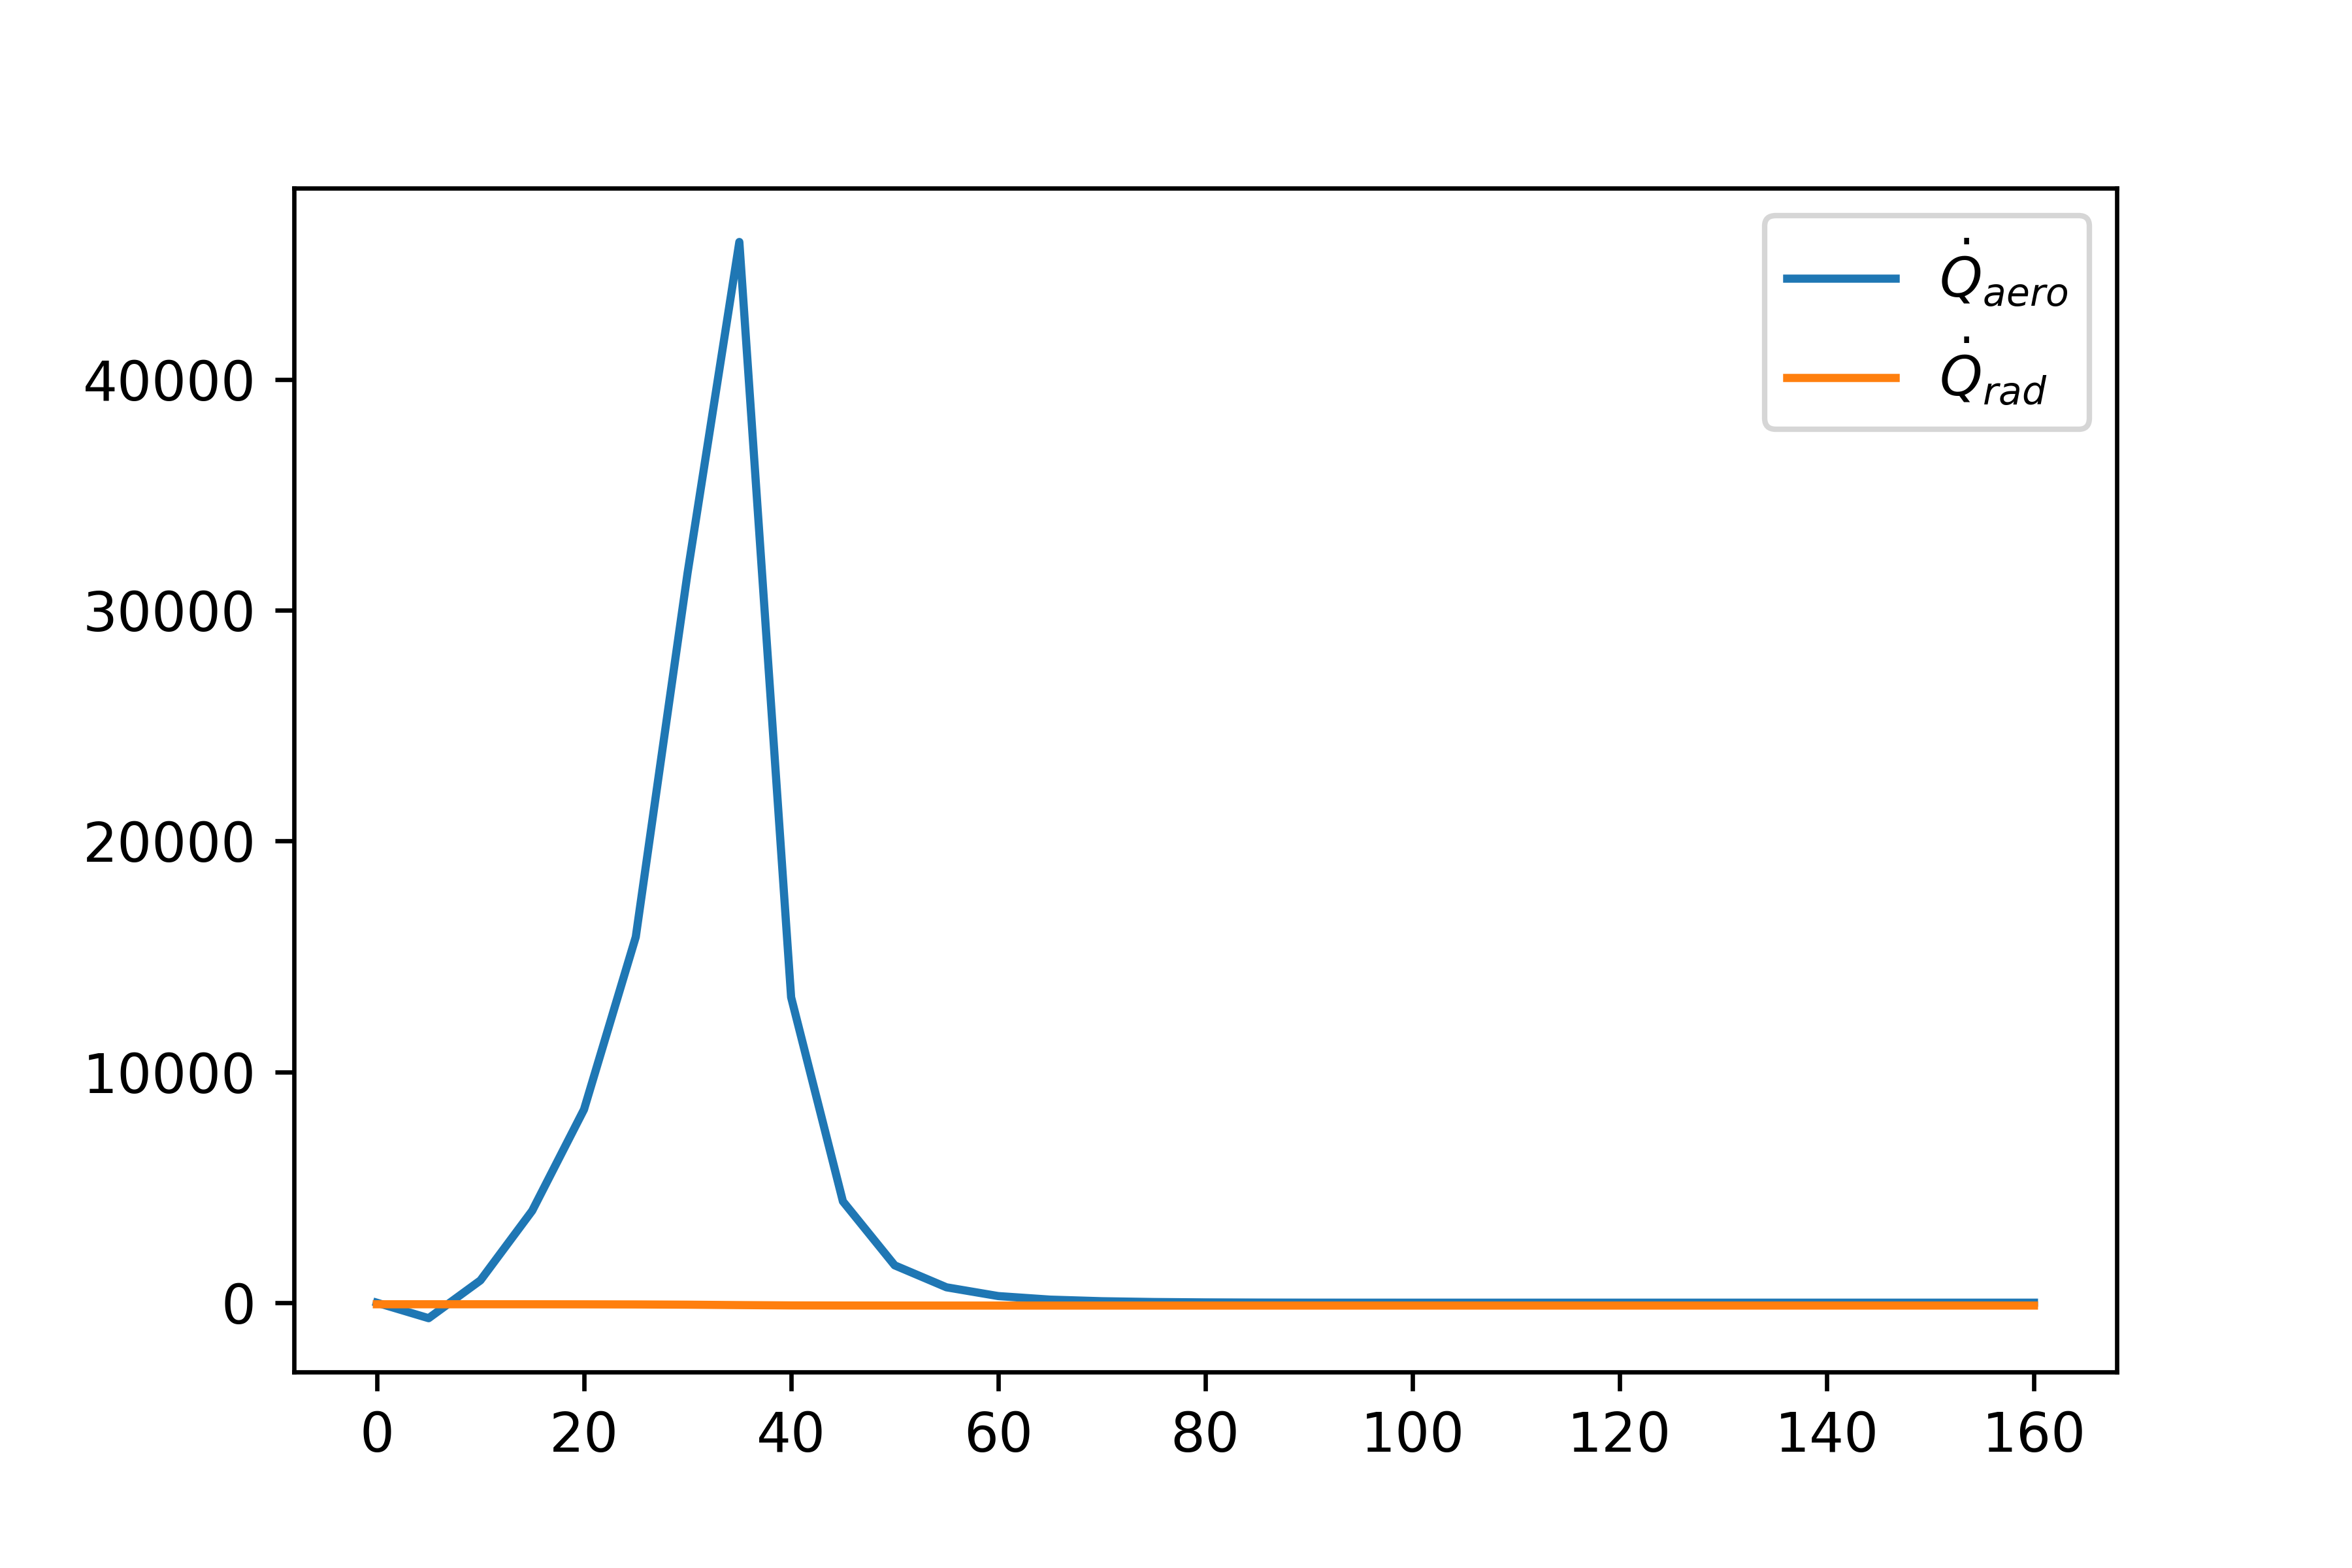
\includegraphics[width=\linewidth]{flux.png}
                \caption{$\dot{Q}_{aero}$ and $\dot{Q}_{rad}$ fluxes over time}
            \end{figure}

            This is explained by figure \ref{fig:flux}: the vast majority of the 
            total heat flux at the skin of the rocket is due to aerodynamic
            effects, with the peak of the aerodynamic flux occuring generally at 
            the same time as the peak mach number. This would seem to be a
            reasonable result. Considering the fixed-vehicle frame of reference,
            as air particles encounter the tip of the nosecone at higher speeds, 
            they will have more kinetic energy, all of which will be transfered 
            to the nosecone, increasing the kinetic energy of it's constituent 
            particles and so increasing it's temperature more than at slower
            velocities. Since we expect the heating of the nosecone to be 
            positively related to the stagnation temperature, we can expect
            higher aerodynamic fluxes at higher speeds. 
            




            



    \onecolumn
    \begin{appendices}
        \section{Atmospheric Models}
            \label{appendix:a}
            \subsection{Air Pressure as a function of Altitude}
                Air pressure $P_0$ as a funciton of altitude $s$ [reference]
                    \[P_0(s)=\begin{cases}
                    \exp{\left(4.43165\cdot10^{-14}s^3-2.28553\cdot10^{-9}s^2-1.14097\cdot10^{-4}s+6.95109\right)} & 0\textrm{km}<s\leq 25\textrm{km}\\
                    \exp{\left(-2.28179\cdot10^{-14}s^3+3.34063\cdot10^-9s^2-2.84655\cdot10^{-4}s+8.73033\right)} & 25\textrm{km} < s \leq 75\textrm{km}\\
                    \exp{\left(4.44813\cdot10^{-14}s^3-1.13434\cdot10^-9s^2+7.62651\cdot10^{-4}s-15.5981\right)} & 75\textrm{km} < s \leq 120\textrm{km}
                \end{cases}\]
            \subsection{Air Density as a function of Altitude}
                Air pressure $\rho_0$ as a function of altidue $s$ [reference]
                \[\rho_0(s)=\begin{cases}
                    \exp{\left(4.88158\cdot10^{-18}s^4-1.808\cdot10^{-13}s^3+2.432\cdot10^{-11}s^2-9.693\cdot10^{-5}s+0.1922\right)} &  0\textrm{km}<s\leq 25\textrm{km}\\
                    \exp{\left(-6.034\cdot10^{-19}s^4-1.035\cdot10^{-13}s^3-5.746\cdot10^{-9}s^2-2.21\cdot10^{-5}-0.396\right)} &  25\textrm{km}<s\leq 75\textrm{km}\\
                    \exp{\left(-1.004\cdot10^{-18}s^4+4.440\cdot10^{-13}s^3-7.137\cdot10^{-8}s^2+4.773\cdot10^{-5}-121.84\right)} &  75\textrm{km}<s\leq 120\textrm{km}
                \end{cases}\]
            \subsection{Air Temperature as a function of Altitude}
                Air Temperature, $T_0$, as a function of altitude $s$ [ref]

                \[T_0(s)=\begin{cases}
                    287.954-5.03015\cdot10^{-3}s-1.2859\cdot10^{-7}s^2 & 0\textrm{km}<s\leq 10\textrm{km}\\
                    225.15 & 10\textrm{km}<s\leq 23\textrm{km}\\
                    242.057-2.33854\cdot10^{-3}s+7.08133\cdot10^{-8}s^2 & 23\textrm{km}<s\leq 42\textrm{km}\\
                    -534.104+3.95468\cdot10^{-2}s-6.0177\cdot10^{-7}s^2+2.71838\cdot10^{-12}s^3 & 42\textrm{km}<s\leq 81.5\textrm{km}\\
                    867.12-9.78603\cdot10^{-3}s-5.75164\cdot10^{-8}s^2+8.81316\cdot10^{-13}s^3 &  81.5\textrm{km}<s\leq 120\textrm{km}
                \end{cases}\]
            \subsection{Dynamic Viscocity of Air as a function of Temperature}
                Dynamic Viscocity of Air, $\mu$, as a function of Temperature $T_0$ [reference]
                
                \[\mu(T_0)=-1.00\cdot10^{-5}-1.47\cdot10^{-9}T+1.68\cdot10^{-6}T^{\frac{1}{2}}\]

            \subsection{Thermal Conductivity of Air as a funciton of Temperature}
                Thermal Conductivity of Air, $k$, as a funciton of Temperature $T_0$ [ref]
                \[k(T_0)=-1.29\cdot10^{-2}+2.43\cdot10^{-5}T-3.39\cdot10^{-9}T^2+1.88\cdot10^{-3}T^{\frac{1}{2}}\]

        \section{Simulation Constants}
        \label{appendix:b}
    \end{appendices}

















\end{document}